%%=============================================================================
%% Resultaten
%%=============================================================================

\chapter{\IfLanguageName{dutch}{Resultaten}{Results}}
\label{ch:resultaten}

\section{\IfLanguageName{dutch}{Inleiding}{Preface}}
\label{sec:resultaten-inleiding}
Na het uitvoeren van de code zoals besproken in Hoofdstuk\ref{ch:methodologie} werd er een csv\footnote{https://docs.google.com/spreadsheets/d/1vGC7rQ9PlnfjhAAsU6fJdlmlrZMXW1S3uCMdqmFghqI} gegenereerd waarbij voor iedere afbeelding in de dataset 3 labels werden opgehaald bij de respectievelijke API's.

Op basis van deze csv werd voor iedere label een score vastgelegd zoals besproken in Sectie~\ref{sec:scoren-van-labels}. Daarnaast werd voor ieder gevonden label aangeduid of de threshold van 75\% zekerheidsgraad gehaald werd, de volledige resultaten van de scoring kunnen teruggevonden worden in deze\footnote{https://docs.google.com/spreadsheets/d/1oCs-aDkhPV2lCayjLyzUPF0SlAUZ7vMjzD4DYuIluyE} Google Sheet. In de sheet kan men ook de aggregatie van de resultaten en grafieken terugvinden.

In de eerste sectie van dit hoofdstuk worden de resultaten besproken waarbij labels met een zekerheidsgraad onder de threshold genegeerd werden. In de volgende sectie worden de volledige resultaten van het onderzoek besproken en wordt de impact van de threshold per computer vision API verder toegelicht. Ten slotte wordt de peformantie van iedere API besproken en wordt er een besluit getrokken in functie van de onderzoeksvraag.

\section{\IfLanguageName{dutch}{Resultaten met thresholding}{Results with thresholding on confidence}}
\label{sec:resultaten-met-thresholding}
In de genormaliseerde staafdiagram op Figuur~\ref{fig:resultswiththresholding} worden het aantal resultaten per score van iedere computer vision API afgebeeld, waarbij de labels met een zekerheidsgraad onder 75\% werden genegeerd. Figuur~\ref{fig:resultswiththresholdingnotstacked} beeldt dezelfde data af maar in absolute waardes.

\begin{figure}
    \centering    
    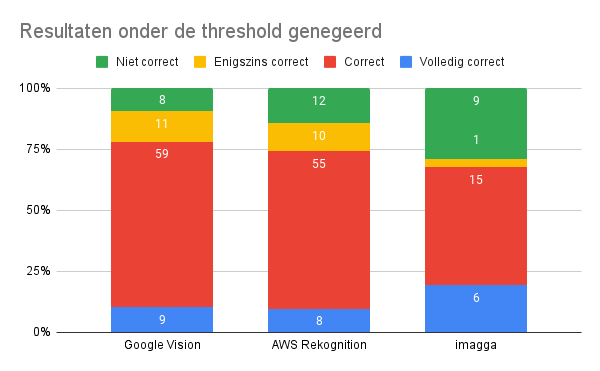
\includegraphics[width=\textwidth]{resultswiththresholding}
    \caption{Resultaten label-herkenning per API, met thresholding}
    \label{fig:resultswiththresholding}
\end{figure}

\begin{figure}
    \centering    
    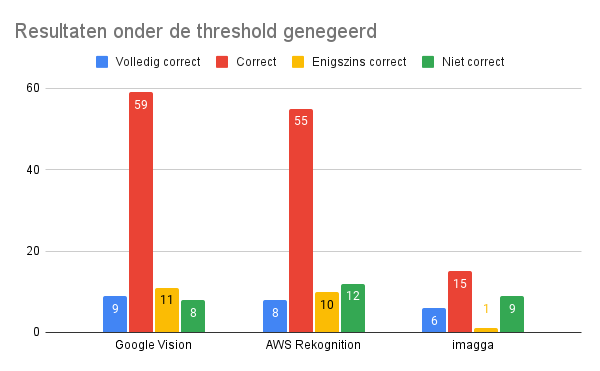
\includegraphics[width=\textwidth]{resultswiththresholdingnotstacked}
    \caption{Resultaten label-herkenning per API, met thresholding niet genormaliseerd}
    \label{fig:resultswiththresholdingnotstacked}
\end{figure}

Bij zowel Google Vision als AWS Rekognition zijn de resultaten gelijkaardig, imagga scoort significant verschillend. Aangezien de resultaten van Google Vision en AWS Rekognition dicht bij elkaar liggen worden deze naast elkaar besproken. Bij beide API's is het grootste deel van de gevonden labels 'correct'. Dit betekent dat de label correct was voor de afbeelding maar niet in de originele dataset vervat zat. Verder wijken ook de scores van van 'volledig correct' en 'engiszins correct' niet van elkaar significant af. Bij Google Vision werden er 8 labels - of 9,2\% van het totaal- als 'niet correct' gepunt, AWS Rekognition scoort hier 12 verkeerde labels of 14,12\% van het totaal. Een verschil minder dan 5\% is niet significant maar kan een trend voorspellen.

In Figuur~\ref{fig:resultsthresholding} wordt het aantal labels afgebeeld dat de threshold-zekerheidsgraad niet haalde, opnieuw zien we een niet significant verschil tussen Google Vision en AWS Rekognition. Bij Google Vision vielen 3 labels of 3,3\% van het totaal onder de threshold, bij AWS Rekognition is dat 5 labels of 5,6\% van het totaal. Men kan stellen dat de resultaten over de hele lijn sterk gelijkaardig zijn tussen Google Vision en AWS Rekognition, met de mogelijkheid dat Google Vision iets beter scoort.

\begin{figure}
    \centering    
    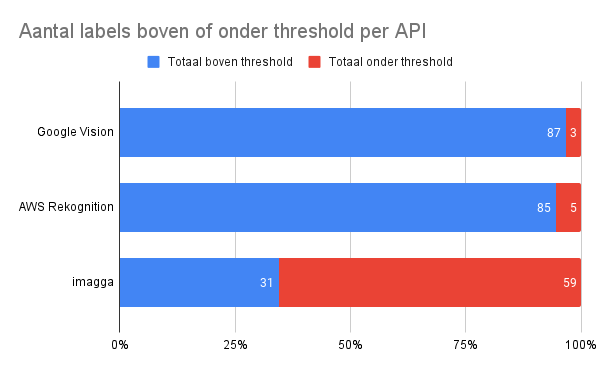
\includegraphics[width=\textwidth]{resultsthresholding}
    \caption{Aantal labels boven of onder de threshold per API}
    \label{fig:resultsthresholding}
\end{figure}

De resultaten van imagga geven een ander beeld, bij Figuur~\ref{fig:resultswiththresholdingnotstacked} is op het eerste zich duidelijk dat er minder resultaten beschikbaar zijn als bij Google Vision of AWS Rekognition. Dit komt omdat 59 van de 90 labels (of 65,6\%) onder de threshold vallen, dit zorgt voor slechts 31 resultaten die geanalyseerd kunnen worden.

Opvallend is dat voor imagga het aantal labels met 'volledig correct' een significant hoger percentage (19,35\%) van het totaal omvat als voor Google Vision (10,34\%) of AWS Rekognition (9,41\%). Verder heeft imagga slechts 1 'engiszins correct' label. 9 labels of 29,03\% van het totaal werden gescoord als 'niet correct', dit is een significant verschil met de 'niet correct' scores van Google Vision en AWS Rekognition. Aangezien er voor imagga procentueel gezien veel labels als 'volledig correct' en 'niet correct' werden aangeduid maar weinig labels als 'enigszins correct' kan men stellen dat het model ofwel zeer correct is, ofwel volledig verkeerd is. 15 labels of 48,39\% van het totaal werden voor imagga als 'correct' aangeduid, opnieuw is dat een significant lager percentage vergeleken met Google Vision (67,8\%) en AWS Rekognition (64,7\%).

Verder viel bij het analyseren van de resultaten op dat imagga de enige API is die zekerheidsgraden van 100\% terug geeft, opnieuw kan men stellen dat imagga ofwel heel zeker is of helemaal niet zeker. De zekerheidsgraden van Google Vision en AWS Rekognition bevinden zich meestal tussen 85\% en 99.9\%.

\section{\IfLanguageName{dutch}{Resultaten zonder thresholding}{Results without thresholding}}
\label{sec:resultaten-zonder-thresholding}
In Figuur~\ref{fig:resultswithoutthresholding} worden de opgetelde scores per API genormaliseerd afgebeeld, zonder dat de scores onder de threshold werden genegeerd.

Het verschil in scores tussen Google Vision en AWS Rekognition is opnieuw niet significant, dit is logisch te verklaren omdat bij beide API's slechts enkele labels onder de threshold vielen. Bij imagga wordt er echter belangrijke significante verschillen opgemerkt, er zijn 27 meer 'correct' labels en 26 meer 'niet correct' labels. Procentueel gezien stijgt 'niet correct' met 9,1\% en daalt 'volledig correct' met 11,6\% de andere scores zijn niet significant verschillend.

Er kan gesteld worden dat imagga veruit het meest terughoudend is met de zekerheidgraad, een correct manier van labelen aangezien het accepteren van een lagere zekerheidsgraad procentueel gezien tot meer verkeerde resultaten leidt.

\begin{figure}
    \centering    
    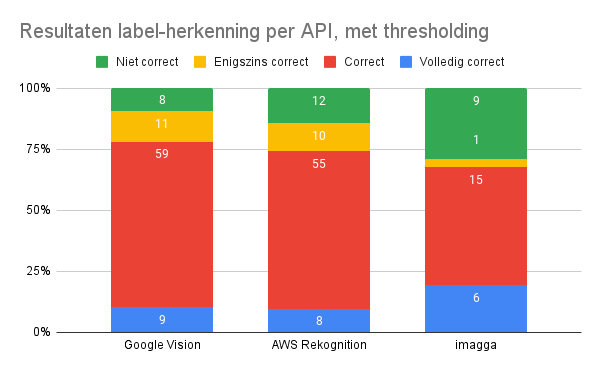
\includegraphics[width=\textwidth]{resultswithoutthresholding}
    \caption{Resultaten label-herkenning per API, zonder thresholding}
    \label{fig:resultswithoutthresholding}
\end{figure}

\section{\IfLanguageName{dutch}{Snelheid per API}{Speed per api}}
\label{sec:snelheid-per-api}
Alhoewel snelheid van verwerking geen belangrijk doel is in de use-case van deze Bachelorproef wordt ze toch kort geanalyseerd als bijkomstige informatie. 
Van iedere call werd bijgehouden hoe snel labels geretourneerd worden, deze data werd verwerkt tot gemiddeldes:

\begin{enumerate}
    \item Classificeren van afbeeldingen: terminologie en technieken
    \item Bespreking belangrijkste stromingen binnen machine learning
    \item Computer vision: hoe wordt classificatie en machine learning gecombineerd
\end{enumerate}

\section{\IfLanguageName{dutch}{Besluit}{Resolution}}
\label{sec:besluit}